\documentclass[11pt]{article}
\usepackage{aa}

\begin{document}
\zestaw{0}{Notacja asymptotyczna, liczby harmoniczne, rekurencje}

\begin{teoria}[Jak czytać ten dokument]
Każde zadanie ma: przepisaną \textbf{treść} (szare pudełko), potrzebną
\textbf{teorię} (niebieskie), \textbf{intuicję} (żółte), \textbf{rozwiązanie
formalne} i~\textbf{odpowiedź} (zielone). Wszystkie wzory zwarte z~tego zestawu
zostały dodatkowo sprawdzone numerycznie skryptem \texttt{weryfikacja/aa00.py}.
Przyjmujemy $\lg = \log_2$, $\ln = \log_e$.
\end{teoria}

% =====================================================================
\section{Notacja asymptotyczna --- teoria}

\begin{definicja}[Notacje $\O$, $\Omega$, $\Theta$, $o$, $\sim$]
Dla funkcji $f,g\colon\N\to\R$, $g>0$ od pewnego miejsca:
\begin{itemize}
  \item $f(n) = \O(g(n))$ $\iff$ $\exists\, C>0,\ n_0\ \forall n\ge n_0:\ |f(n)|\le C\,g(n)$
        („$f$ rośnie co najwyżej tak szybko jak $g$”);
  \item $f(n) = \Omega(g(n))$ $\iff$ $\exists\, c>0,\ n_0\ \forall n\ge n_0:\ f(n)\ge c\,g(n)$;
  \item $f(n) = \Theta(g(n))$ $\iff$ $f=\O(g)$ i $f=\Omega(g)$;
  \item $f(n) = o(g(n))$ $\iff$ $f(n)/g(n)\to 0$ („$g$ rośnie istotnie szybciej”);
  \item $f(n) \sim g(n)$ $\iff$ $f(n)/g(n)\to 1$.
\end{itemize}
\end{definicja}

\begin{definicja}[$\O$ wewnątrz wzorów]
Zapis $\O(g(n))$ wewnątrz wyrażenia oznacza \emph{jakąś} funkcję $h(n)$, dla
której $h(n)=\O(g(n))$. Równość z~$\O$ po obu stronach, np.
$e^{1+\O(1/n)} = e+\O(1/n)$, czytamy \emph{jednostronnie}: każda funkcja postaci
z~lewej strony jest też postaci z~prawej strony (to jest „$\subseteq$”, nie „$=$”).
\end{definicja}

\begin{definicja}[Błąd względny]
Oszacowanie $f(n)$ przez $g(n)$ ma \emph{błąd względny} $\O(\varepsilon(n))$,
jeśli $f(n) = g(n)\bigl(1+\O(\varepsilon(n))\bigr)$, czyli
$\bigl|\frac{f(n)-g(n)}{g(n)}\bigr| = \O(\varepsilon(n))$.
\end{definicja}

\begin{fakt}[Rozwinięcia, których używamy]\label{fakt:rozw}
Gdy $x\to 0$:
\begin{gather*}
e^{x} = 1 + x + \O(x^2) = 1+\O(x),\\
\ln(1+x) = x - \frac{x^2}{2} + \O(x^3) = x+\O(x^2).
\end{gather*}
Precyzyjnie: dla $|x|\le 1$ mamy $|e^x-1|\le |x|e^{|x|}\le e|x|$, a dla
$|x|\le\frac12$ mamy $|\ln(1+x)-x|\le x^2$. (Oba wynikają z~szeregów Taylora.)
\end{fakt}

\begin{twierdzenie}[Wzór Stirlinga]\label{tw:stirling}
\[
n! = \sqrt{2\pi n}\,\Bigl(\frac{n}{e}\Bigr)^{n}\Bigl(1+\O\bigl(\tfrac1n\bigr)\Bigr).
\]
\end{twierdzenie}

\begin{fakt}[Prosta dolna granica na silnię]\label{fakt:silnia}
Dla $k\ge 1$: $k!\ge (k/e)^k$. \emph{Dowód:} $e^k=\sum_{j\ge0}k^j/j!\ \ge\ k^k/k!$.
\end{fakt}

\begin{intuicja}
Porównując szybkość wzrostu dwóch dodatnich funkcji, najwygodniej porównać ich
\textbf{logarytmy}: jeśli $\ln f(n) - \ln g(n)\to+\infty$, to
$f(n)/g(n) = e^{\ln f - \ln g}\to\infty$, czyli $f$ rośnie szybciej
($g=o(f)$). Logarytm zamienia potęgi na iloczyny, a~iloczyny na sumy --- dużo
łatwiej się to porównuje.
\end{intuicja}

% ---------------------------------------------------------------------
\section{Zadanie 1. Która funkcja rośnie szybciej?}
\begin{tresc}
Która z poniższych funkcji rośnie szybciej:
(a) $n^{\ln n}$ czy $(\ln n)^n$?\quad
(b) $\floor{\ln n}!$ czy $n^{\ln\ln\ln n}$?\quad
(c) $\lg(\lgs n)$ czy $\lgs(\lg n)$?
\end{tresc}

\begin{teoria}[Logarytm iterowany $\lgs$]
\begin{definicja}
$\lgs x = 0$ dla $x\le 1$ oraz $\lgs x = 1+\lgs(\lg x)$ dla $x>1$. Innymi słowy
$\lgs x$ to liczba logarytmowań, po których wynik spadnie do $\le 1$.
\end{definicja}
Przykłady: $\lgs 2=1$, $\lgs 4=2$, $\lgs 16=3$, $\lgs 65536=4$,
$\lgs 2^{65536}=5$. Funkcja ta rośnie \emph{niewyobrażalnie} wolno, ale
$\lgs n\to\infty$. Bezpośrednio z~definicji: $\lgs(\lg n)=\lgs n-1$ dla $n>1$.
\end{teoria}

\subsection*{(a) $n^{\ln n}$ vs $(\ln n)^n$}
\begin{intuicja}
$n^{\ln n}$ to „$n$ do potęgi logarytm” --- funkcja quasi-wielomianowa.
$(\ln n)^n$ ma w~wykładniku \emph{całe} $n$, więc jest ponad-wykładnicza.
\end{intuicja}
\formalnie
$\ln\bigl(n^{\ln n}\bigr) = (\ln n)^2$ oraz $\ln\bigl((\ln n)^n\bigr) = n\ln\ln n$.
Różnica
\begin{align*}
n\ln\ln n - (\ln n)^2 &= n\ln\ln n\Bigl(1 - \frac{(\ln n)^2}{n\ln\ln n}\Bigr)\\
&\xrightarrow{n\to\infty}+\infty,
\end{align*}
bo $(\ln n)^2/n\to 0$ (logarytm w~dowolnej potędze rośnie wolniej niż $n$),
a $\ln\ln n\ge 1$ dla $n\ge e^e$. Zatem $\frac{(\ln n)^n}{n^{\ln n}}\to\infty$.
\begin{odpowiedz}
$(\ln n)^n$ rośnie szybciej: $n^{\ln n} = o\bigl((\ln n)^n\bigr)$.
\end{odpowiedz}

\subsection*{(b) $\floor{\ln n}!$ vs $n^{\ln\ln\ln n}$}
\begin{intuicja}
Podstawmy $m=\ln n$. Wtedy pierwsza funkcja to około $m!\approx (m/e)^m$,
czyli $e^{m\ln m - m}$, a druga to $e^{m\ln\ln m}$. Porównujemy $m\ln m$
z~$m\ln\ln m$ --- wygrywa $\ln m$, bo $\ln m \gg \ln\ln m$.
\end{intuicja}
\formalnie
Niech $m=\ln n$ i $k=\floor{m}\ge m-1$. Z~Faktu~\ref{fakt:silnia}:
\[
\ln(k!) \ge k\ln k - k \ge (m-1)\ln(m-1) - m .
\]
Dla $m\ge 2$ mamy $\ln(m-1)=\ln m+\ln(1-\tfrac1m)\ge \ln m-\tfrac2m$, więc
$\ln(k!)\ge (m-1)\ln m - 2 - m$. Natomiast
$\ln\bigl(n^{\ln\ln\ln n}\bigr)=\ln n\cdot\ln\ln\ln n = m\ln\ln m$. Stąd
\begin{align*}
\ln\floor{\ln n}! - \ln n^{\ln\ln\ln n} &\ge m\bigl(\ln m - \ln\ln m - 1\bigr) - \ln m - 2\\
&\xrightarrow{m\to\infty} +\infty,
\end{align*}
bo $\ln m - \ln\ln m - 1\to\infty$.
\begin{odpowiedz}
$\floor{\ln n}!$ rośnie szybciej: $n^{\ln\ln\ln n} = o\bigl(\floor{\ln n}!\bigr)$.
\end{odpowiedz}

\subsection*{(c) $\lg(\lgs n)$ vs $\lgs(\lg n)$}
\begin{intuicja}
$\lgs(\lg n)$ to po prostu $\lgs n - 1$ (jedno logarytmowanie „zużyliśmy”
z~góry). Porównujemy więc $\lg m$ z~$m-1$ dla $m=\lgs n\to\infty$ --- liniowa
funkcja bije logarytm.
\end{intuicja}
\formalnie
Dla $n>1$ z~definicji $\lgs(\lg n)=\lgs n-1$. Niech $m=\lgs n$; $m\to\infty$
gdy $n\to\infty$. Wtedy
$\dfrac{\lg(\lgs n)}{\lgs(\lg n)} = \dfrac{\lg m}{m-1}\to 0.$
\begin{odpowiedz}
$\lgs(\lg n)$ rośnie szybciej: $\lg(\lgs n) = o\bigl(\lgs(\lg n)\bigr)$.
\end{odpowiedz}

% ---------------------------------------------------------------------
\section{Zadanie 2. Oszacowanie \texorpdfstring{$\bigl(n+2+\O(n^{-1})\bigr)^n$}{(n+2+O(1/n))\textasciicircum n}}
\begin{tresc}
Podaj oszacowanie asymptotyczne wyrażenia $\bigl(n+2+\O(n^{-1})\bigr)^n$
z~błędem względnym rzędu $\O(n^{-1})$.
\end{tresc}

\begin{intuicja}
Wyciągamy $n$ przed nawias: $n^n\bigl(1+\frac2n+\dots\bigr)^n$. Pamiętamy, że
$\bigl(1+\frac xn\bigr)^n\to e^x$, więc spodziewamy się $e^2 n^n$. Trzeba
tylko pilnować, ile kosztują „śmieci” $\O(n^{-2})$: przemnożone przez
wykładnik $n$ dają $\O(n^{-1})$ --- dokładnie tyle, ile wolno.
\end{intuicja}
\formalnie
\begin{align*}
\bigl(n+2+\O(n^{-1})\bigr)^n &= n^n\Bigl(1+\underbrace{\tfrac2n+\O(n^{-2})}_{=:x}\Bigr)^n\\
&= n^n \exp\bigl(n\ln(1+x)\bigr).
\end{align*}
Ponieważ $x=\O(1/n)\to0$, z~Faktu~\ref{fakt:rozw}:
$\ln(1+x) = x+\O(x^2) = \tfrac2n + \O(n^{-2}) + \O(n^{-2}) = \tfrac2n+\O(n^{-2})$.
Mnożymy przez $n$: $n\ln(1+x) = 2+\O(n^{-1})$. Zatem
\begin{align*}
n^n\exp\bigl(2+\O(n^{-1})\bigr) &= e^2n^n\, e^{\O(n^{-1})}\\
&= e^2 n^n\bigl(1+\O(n^{-1})\bigr),
\end{align*}
gdzie w~ostatnim kroku znów użyliśmy $e^y=1+\O(y)$ dla $y\to0$.
\begin{odpowiedz}
$\bigl(n+2+\O(n^{-1})\bigr)^n = e^2 n^n\bigl(1+\O(n^{-1})\bigr) = e^2n^n+\O(n^{n-1})$.
\end{odpowiedz}

% ---------------------------------------------------------------------
\section{Zadanie 3. Sprawdzenie oszacowań}
\begin{tresc}
Sprawdź, czy poniższe oszacowania są prawdziwe przy $n\to\infty$:\\
(a) $e^{(1+\O(1/n))^2} = e+\O(1/n)$,\qquad
(b) $n! = \O\Bigl(\bigl((1-1/n)^n n\bigr)^n\Bigr)$.
\end{tresc}

\subsection*{(a)}
\begin{intuicja}
$(1+\text{mało})^2 = 1+\text{mało}$, a $e^{1+\text{mało}} = e\cdot e^{\text{mało}}
= e(1+\text{mało})$. „Mało” cały czas jest rzędu $1/n$.
\end{intuicja}
\formalnie
Niech $h(n)=\O(1/n)$, tzn. $|h(n)|\le C/n$ dla $n\ge n_0$. Wtedy
$(1+h)^2 = 1 + 2h + h^2$ i $|2h+h^2|\le 2C/n + C^2/n^2\le (2C+C^2)/n$, czyli
$(1+h)^2 = 1+\O(1/n)$. Dalej
\[
e^{(1+h)^2} = e\cdot e^{\O(1/n)} = e\bigl(1+\O(1/n)\bigr) = e+\O(1/n),
\]
gdzie korzystamy z~$|e^y-1|\le e|y|$ dla $|y|\le1$ (Fakt~\ref{fakt:rozw}).
\begin{odpowiedz}
(a) \textbf{Prawda.}
\end{odpowiedz}

\subsection*{(b)}
\begin{intuicja}
$(1-1/n)^n\approx 1/e$, więc prawa strona to w~przybliżeniu $(n/e)^n$.
Ze Stirlinga $n!\approx\sqrt{2\pi n}(n/e)^n$ --- jest większe o~czynnik
$\sqrt n$, który dąży do nieskończoności. Trzeba jednak uważać:
$(1-1/n)^n$ to nie dokładnie $1/e$, a podnosimy to jeszcze do potęgi $n$,
więc błąd może się „rozdmuchać”. Liczymy dokładniej i okazuje się, że daje
on tylko stały czynnik $e^{-1/2}$.
\end{intuicja}
\formalnie
Z~szeregu $\ln(1-x) = -x-\frac{x^2}{2}-\O(x^3)$ dla $x=1/n$:
\begin{align*}
\ln\Bigl(\bigl((1-\tfrac1n)^n n\bigr)^n\Bigr) &= n\ln n + n^2\ln(1-\tfrac1n)\\
&= n\ln n - n - \tfrac12 + \O(\tfrac1n).
\end{align*}
Stąd prawa strona to $R(n) = n^n e^{-n} e^{-1/2}\bigl(1+\O(1/n)\bigr)$.
Ze wzoru Stirlinga (Tw.~\ref{tw:stirling})
\begin{align*}
\frac{n!}{R(n)} &= \frac{\sqrt{2\pi n}\,(n/e)^n(1+\O(1/n))}{e^{-1/2}(n/e)^n(1+\O(1/n))}\\
&= \sqrt{2\pi e\, n}\,\bigl(1+\O(1/n)\bigr)\xrightarrow{n\to\infty}\infty.
\end{align*}
Iloraz nie jest ograniczony, więc $n!\neq\O(R(n))$.
\begin{odpowiedz}
(b) \textbf{Fałsz.} Zachodzi $n!=\Theta\bigl(\sqrt n\cdot((1-1/n)^n n)^n\bigr)$.
\end{odpowiedz}

% ---------------------------------------------------------------------
\section{Zadanie 4. Asymptotyka liczb Catalana}
\begin{tresc}
Wykorzystując wzór asymptotyczny Stirlinga, znajdź oszacowanie asymptotyczne
$n$-tej liczby Catalana: $C_n = \frac{1}{n+1}\binom{2n}{n}$.
\end{tresc}

\begin{teoria}[Liczby Catalana]
$C_n$ liczy m.in.\ poprawne nawiasowania z~$n$ par nawiasów, drzewa binarne
o~$n$ węzłach, ścieżki Dycka. $C_0,C_1,\ldots = 1,1,2,5,14,42,\ldots$
\end{teoria}

\begin{intuicja}
$\binom{2n}{n}$ to środkowy (największy) z~$2n+1$ współczynników, które
sumują się do $4^n$. Więc jest „trochę mniejszy” od $4^n$ --- o~czynnik
$\sqrt{\pi n}$ (rozkład dwumianowy ma szerokość $\sim\sqrt n$). Dzielenie przez
$n+1$ daje jeszcze jedno $n$ w~mianowniku.
\end{intuicja}
\formalnie
Ze wzoru Stirlinga dla $(2n)!$ i $n!$:
\begin{align*}
\binom{2n}{n} = \frac{(2n)!}{(n!)^2}
&= \frac{\sqrt{4\pi n}\,(2n/e)^{2n}\bigl(1+\O(\frac1n)\bigr)}{2\pi n\,(n/e)^{2n}\bigl(1+\O(\frac1n)\bigr)^2}\\
&= \frac{4^n}{\sqrt{\pi n}}\Bigl(1+\O\bigl(\tfrac1n\bigr)\Bigr),
\end{align*}
bo $(2n/e)^{2n}/(n/e)^{2n} = 2^{2n} = 4^n$ oraz $\frac{1+\O(1/n)}{(1+\O(1/n))^2} = 1+\O(1/n)$.
Ponadto $\frac{1}{n+1} = \frac1n\cdot\frac{1}{1+1/n} = \frac1n\bigl(1+\O(\frac1n)\bigr)$.
\begin{odpowiedz}
$C_n = \dfrac{4^n}{\sqrt{\pi}\, n^{3/2}}\Bigl(1+\O\bigl(\tfrac1n\bigr)\Bigr)$, \quad w~szczególności $C_n\sim \dfrac{4^n}{\sqrt\pi\,n^{3/2}}$.
\end{odpowiedz}

% =====================================================================
\section{Liczby harmoniczne --- teoria}
\begin{definicja}
$n$-ta liczba harmoniczna to $H_n = \sum_{k=1}^n \frac1k = 1+\frac12+\dots+\frac1n$, $H_0=0$.
\end{definicja}
Liczby harmoniczne pojawiają się w~analizie algorytmów bardzo często (np.\
średni czas Quicksorta to $\approx 2nH_n$). Najważniejszy fakt to
$H_n = \ln n + \O(1)$ --- dokładniej $H_n = \ln n + \gamma + \O(1/n)$, gdzie
$\gamma\approx 0{,}5772$ to stała Eulera--Mascheroniego.

% ---------------------------------------------------------------------
\section{Zadanie 5. \texorpdfstring{$H_n$}{H(n)} nie jest liczbą całkowitą}
\begin{tresc}
Pokaż, że $n$-ta liczba harmoniczna $H_n=\sum_{k=1}^n\frac1k$ jest liczbą
niecałkowitą dla każdej liczby naturalnej $n>1$.
\end{tresc}

\begin{intuicja}
Patrzymy na potęgi dwójki w~mianownikach. Wśród $1,2,\ldots,n$ jest
\emph{dokładnie jedna} liczba podzielna przez największą możliwą potęgę
dwójki $2^k\le n$ --- sama $2^k$. Jeśli sprowadzimy wszystko do wspólnego
mianownika „prawie”, tzn. z~potęgą dwójki o~jeden za małą, to wszystkie
składniki staną się całkowite \emph{oprócz} $\frac{1}{2^k}$, który da połówkę.
Liczba całkowita $+\frac12$ nie jest całkowita.
\end{intuicja}
\formalnie
Niech $n\ge2$ i $k=\floor{\lg n}\ge 1$, czyli $2^k\le n<2^{k+1}$. Każdą liczbę
$j\in\{1,\dots,n\}$ zapisujemy jako $j=2^{a_j}o_j$, $o_j$ nieparzyste.

\textit{Obserwacja:} $a_j\le k-1$ dla wszystkich $j\ne 2^k$. Istotnie, $a_j\le k$
bo $2^{a_j}\le j\le n<2^{k+1}$; a~gdyby $a_j=k$ i $j\ne 2^k$, to $o_j\ge3$
i~$j\ge 3\cdot2^k>n$ --- sprzeczność.

Niech $P$ będzie iloczynem wszystkich liczb nieparzystych $\le n$ ($P$ jest
nieparzyste) i~$M=2^{k-1}P$. Wtedy
\begin{align*}
M\cdot H_n &= \sum_{\substack{j\le n\\ j\ne 2^k}} \frac{2^{k-1}P}{2^{a_j}o_j} \;+\; \frac{2^{k-1}P}{2^k}\\
&= (\text{liczba całkowita}) + \frac{P}{2},
\end{align*}
bo każdy składnik sumy jest całkowity ($a_j\le k-1$ oraz $o_j\mid P$).
Ponieważ $P$ jest nieparzyste, $\frac P2\notin\Z$, więc $MH_n\notin\Z$.
Gdyby $H_n$ była całkowita, to $MH_n$ też byłoby całkowite. Sprzeczność.\qed
\begin{odpowiedz}
Dla $n>1$ liczba $H_n$ ma w~mianowniku (po skróceniu) czynnik $2^{\floor{\lg n}}$, więc nie jest całkowita.
\end{odpowiedz}

% ---------------------------------------------------------------------
\section{Zadanie 6. \texorpdfstring{$\ln n < H_n < \ln n + 1$}{ln n < H(n) < ln n + 1}}
\begin{tresc}
Udowodnij nierówności: $\ln n < H_n < \ln n+1$ dla $n>1$.
\end{tresc}

\begin{intuicja}
$H_n$ to pole $n$ prostokątów o~szerokości 1 i~wysokości $1/k$. Wykres
$y=1/x$ jest malejący, więc prostokąty „wystają” nad wykres, jeśli stawiamy je
na przedziałach $[k,k+1]$, a~„chowają się” pod wykresem, jeśli stawiamy je na
$[k-1,k]$. Pole pod wykresem to logarytm.
\end{intuicja}

\begin{center}
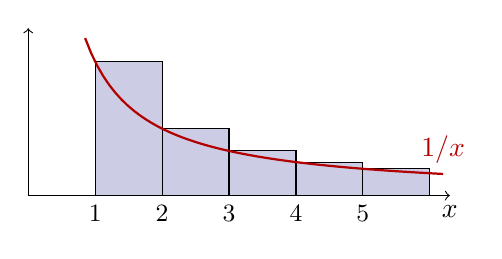
\begin{tikzpicture}[scale=0.85,x=1cm,y=2cm]
  \draw[->] (0,0) -- (6.3,0) node[below]{$x$};
  \draw[->] (0,0) -- (0,1.25);
  \foreach \k in {1,...,5} {
     \draw[fill=NavyBlue!20] (\k,0) rectangle ({\k+1},{1/\k});
     \node[below] at (\k,0) {\small $\k$};
  }
  \draw[thick,domain=0.85:6.2,samples=60,red!70!black] plot (\x,{1/\x}) node[above]{$1/x$};
\end{tikzpicture}\\
{\small Prostokąty $[k,k+1]\times[0,\frac1k]$ leżą nad wykresem $1/x$: $H_n>\int_1^{n+1}\frac{dx}{x}$.}
\end{center}

\formalnie
Funkcja $1/x$ jest ściśle malejąca na $(0,\infty)$, więc dla $k\ge1$:
\[
\int_k^{k+1}\frac{dx}{x} < \frac1k \qquad\text{oraz}\qquad \frac1k<\int_{k-1}^{k}\frac{dx}{x}\quad(k\ge2).
\]
\emph{Dolne ograniczenie.} Sumując pierwszą nierówność dla $k=1,\dots,n$:
$H_n > \int_1^{n+1}\frac{dx}{x} = \ln(n+1) > \ln n$.

\emph{Górne ograniczenie.} Sumując drugą nierówność dla $k=2,\dots,n$ (dla $n>1$
jest co najmniej jeden składnik, więc nierówność jest ostra):
$H_n - 1 < \int_1^{n}\frac{dx}{x} = \ln n$, czyli $H_n<\ln n+1$.\qed

% =====================================================================
\section{Rekurencje --- teoria}

\begin{teoria}[Metoda czynnika sumacyjnego]
Rekurencję liniową pierwszego rzędu
\[
a_n = p_n\, a_{n-1} + q_n
\]
rozwiązujemy, mnożąc obie strony przez taki czynnik $s_n$, żeby
$s_n p_n = s_{n-1}$. Wtedy dla $b_n := s_na_n$ dostajemy
\[
b_n = b_{n-1} + s_nq_n\quad\Longrightarrow\quad b_n = b_{n_0} + \sum_{k=n_0+1}^n s_kq_k,
\]
czyli rekurencja zamienia się w~zwykłą sumę. Czynnik można wziąć
$s_n = 1/(p_np_{n-1}\cdots p_{n_0+1})$ (z~dokładnością do stałej).
\end{teoria}

\begin{definicja}[Potęga krocząca w dół]
$\ff{x}{m} = x(x-1)\cdots(x-m+1)$ ($m$ czynników), $\ff{x}{0}=1$.
Dla całkowitych $0\le x<m$ mamy $\ff{x}{m}=0$. Zachodzi
$\ff{(x+1)}{m+1} = (x+1)\ff{x}{m}$ oraz $\ff{x}{m+1} = \ff{x}{m}(x-m)$.
\end{definicja}

% ---------------------------------------------------------------------
\section{Zadanie 7. Rozwiąż rekurencje}
\begin{tresc}
Rozwiąż poniższe rekurencje:
\begin{enumerate}[label=(\alph*)]
\item $a_0=1$,\quad $a_n=\frac{n}{n+2}a_{n-1}$ dla $n>0$;
\item $a_0=1$,\quad $a_n=a_{n-1}+(-1)^n$ dla $n>0$;
\item $a_1=1$,\quad $a_n=\frac1n\bigl((n-2)a_{n-1}+2\bigr)$ dla $n>1$;
\item $a_1=1$,\quad $a_n=2a_{n-1}+1$ dla $n>1$;
\item $a_0=0$,\quad $a_n=\frac{n+1}{n}a_{n-1}+2$ dla $n>0$;
\item $a_n=0$ dla $n\le4$,\quad $a_n=\frac{n-4}{n}a_{n-1}+12H_n$ dla $n>4$.
\end{enumerate}
\end{tresc}

\subsection*{(a) $a_n=\frac{n}{n+2}a_{n-1}$, $a_0=1$}
\begin{intuicja}
Każdy krok mnoży przez ułamek; iloczyn ułamków $\frac{k}{k+2}$ się „teleskopuje”
--- prawie wszystko się skraca.
\end{intuicja}
\formalnie
Rozwijając, $a_n=\prod_{k=1}^n\frac{k}{k+2} = \frac{1\cdot2\cdots n}{3\cdot4\cdots(n+2)}
= \frac{n!\cdot 2}{(n+2)!} = \frac{2}{(n+1)(n+2)}$.
Sprawdzenie: $a_0=\frac{2}{2}=1$, $a_1=\frac13$ \checkmark. (Formalnie: indukcja,
$\frac{n}{n+2}\cdot\frac{2}{n(n+1)}=\frac{2}{(n+1)(n+2)}$.)
\begin{odpowiedz}$a_n = \dfrac{2}{(n+1)(n+2)}$.\end{odpowiedz}

\subsection*{(b) $a_n=a_{n-1}+(-1)^n$, $a_0=1$}
\formalnie
$a_n = 1+\sum_{k=1}^n(-1)^k$. Suma to $-1$ dla $n$ nieparzystych i~$0$ dla
parzystych (wyrazy łączą się w~pary $-1+1$). Ciąg to $1,0,1,0,\ldots$
\begin{odpowiedz}$a_n=\dfrac{1+(-1)^n}{2}$ ($1$ dla $n$ parzystych, $0$ dla nieparzystych).\end{odpowiedz}

\subsection*{(c) $a_n=\frac1n\bigl((n-2)a_{n-1}+2\bigr)$, $a_1=1$}
\begin{intuicja}
Licząc kilka wyrazów: $a_2=\frac{0+2}{2}=1$, $a_3=\frac{1+2}{3}=1$ --- wygląda na
stałą. Rzeczywiście, jeśli $a_{n-1}=1$, to $a_n=\frac{n-2+2}{n}=1$. Pokażmy
jednak, jak doszłoby się do tego metodą czynnika sumacyjnego (bez zgadywania).
\end{intuicja}
\formalnie
Tu $p_n=\frac{n-2}{n}$. Mnożymy przez $s_n=n(n-1)$: wtedy $s_np_n=(n-1)(n-2)=s_{n-1}$.
Dla $b_n=n(n-1)a_n$:
\begin{gather*}
b_n = b_{n-1} + 2(n-1),\quad b_1=0\\
\Longrightarrow\quad b_n=2\sum_{k=2}^n(k-1)=n(n-1).
\end{gather*}
Zatem $a_n = 1$ dla $n\ge2$, a także $a_1=1$.
\begin{odpowiedz}$a_n=1$ dla wszystkich $n\ge1$.\end{odpowiedz}

\subsection*{(d) $a_n=2a_{n-1}+1$, $a_1=1$}
\begin{intuicja}
To rekurencja wież Hanoi. Dodanie $1$ do obu stron daje czyste podwajanie.
\end{intuicja}
\formalnie
$a_n+1 = 2(a_{n-1}+1)$, $a_1+1=2$, więc $a_n+1=2^n$.
\begin{odpowiedz}$a_n=2^n-1$.\end{odpowiedz}

\subsection*{(e) $a_n=\frac{n+1}{n}a_{n-1}+2$, $a_0=0$}
\formalnie
$p_n=\frac{n+1}{n}$, czynnik $s_n=\frac1{n+1}$ (bo $\frac{1}{n+1}\cdot\frac{n+1}{n}=\frac1n=s_{n-1}$).
Dla $b_n=\frac{a_n}{n+1}$:
\begin{gather*}
b_n=b_{n-1}+\frac{2}{n+1},\quad b_0=0\\
\Longrightarrow\quad b_n = 2\sum_{k=1}^n\frac{1}{k+1} = 2\,(H_{n+1}-1).
\end{gather*}
Sprawdzenie: $a_1=2\cdot0+2=2$, wzór: $2\cdot2\cdot(H_2-1)=2$ \checkmark; $a_2=\frac32\cdot2+2=5$, wzór: $6(\frac12+\frac13)=5$ \checkmark.
\begin{odpowiedz}$a_n = 2(n+1)(H_{n+1}-1) = 2(n+1)H_n - 2n$.\end{odpowiedz}

\subsection*{(f) $a_n=\frac{n-4}{n}a_{n-1}+12H_n$, $a_n=0$ dla $n\le4$}
\begin{intuicja}
Ten sam schemat: czynnik sumacyjny zamienia rekurencję w~sumę
$\sum k(k-1)(k-2)(k-3)H_k$. Takie sumy (wielomian razy $H_k$) liczy się
„sumowaniem przez części” --- dyskretnym odpowiednikiem całkowania przez
części; poniżej podajemy gotowy lemat z~dowodem indukcyjnym. Wynik wyjdzie
rzędu $\frac{12}{5}nH_n\approx 2{,}4\,n\ln n$ (tego typu rekurencje opisują
koszty wariantów Quicksorta).
\end{intuicja}

\begin{lemat}\label{lem:sumaH}
Dla całkowitych $m\ge0$, $n\ge0$:
\[
\sum_{0\le k<n}\ff{k}{m}H_k = \frac{\ff{n}{m+1}}{m+1}\Bigl(H_n-\frac{1}{m+1}\Bigr).
\]
\end{lemat}
\begin{proof}
Indukcja po $n$. Dla $n=0$ obie strony są równe $0$. Krok $n\to n+1$: trzeba
pokazać, że prawa strona wzrasta o~$\ff{n}{m}H_n$. Używając
$\ff{(n+1)}{m+1}=(n+1)\ff nm$, $\ff{n}{m+1}=(n-m)\ff nm$, $H_{n+1}=H_n+\frac1{n+1}$:
\begin{align*}
&\frac{\ff nm}{m+1}\Bigl[(n+1)\Bigl(H_n+\frac{1}{n+1}-\frac{1}{m+1}\Bigr)\\
&\hspace{6em}-(n-m)\Bigl(H_n-\frac1{m+1}\Bigr)\Bigr]\\
&\quad=\frac{\ff nm}{m+1}\Bigl[(m+1)H_n + 1 - \frac{n+1}{m+1}+\frac{n-m}{m+1}\Bigr]\\
&\quad=\frac{\ff nm}{m+1}(m+1)H_n = \ff nmH_n.\qedhere
\end{align*}
\end{proof}

\formalnie
$p_n=\frac{n-4}{n}$; czynnik $s_n=\ff n4=n(n-1)(n-2)(n-3)$, bo
$\ff n4\cdot\frac{n-4}{n} = (n-1)(n-2)(n-3)(n-4)=\ff{(n-1)}{4}$.
Dla $b_n=\ff n4a_n$ mamy $b_4=0$ i
\begin{gather*}
b_n = b_{n-1}+12\,\ff n4H_n\\
\Longrightarrow\quad b_n = 12\sum_{k=5}^n\ff k4H_k.
\end{gather*}
Z~Lematu~\ref{lem:sumaH} ($m=4$, górna granica $n+1$), pamiętając, że wyrazy
$k\le3$ są zerowe, a wyraz $k=4$ to $4!\,H_4 = 24\cdot\frac{25}{12}=50$:
\begin{align*}
\sum_{k=5}^n\ff k4H_k &= \frac{\ff{(n+1)}{5}}{5}\Bigl(H_{n+1}-\frac15\Bigr) - 50\\
&= \frac{(n+1)\ff n4}{5}\Bigl(H_{n+1}-\frac15\Bigr) - 50.
\end{align*}
Dzieląc przez $\ff n4$ i~mnożąc przez 12:
\[
a_n = \frac{12}{5}(n+1)\Bigl(H_{n+1}-\frac15\Bigr) - \frac{600}{\ff n4}.
\]
Używając $(n+1)H_{n+1}=(n+1)H_n+1$ upraszczamy pierwszy składnik:
\[
\tfrac{12}{5}(n+1)H_n+\tfrac{12}{5}-\tfrac{12(n+1)}{25} = \tfrac{12}{5}(n+1)H_n-\tfrac{12(n-4)}{25}.
\]

Sprawdzenie: $n=4$: $\frac{12}{5}\cdot5\cdot\frac{25}{12}-0-\frac{600}{24}=25-25=0$ \checkmark;
$n=5$: z~rekurencji $a_5=12H_5=\frac{137}{5}$, ze wzoru $\frac{72}{5}\cdot\frac{137}{60}-\frac{12}{25}-5=\frac{137}{5}$ \checkmark.
\begin{odpowiedz}
Dla $n\ge4$:
\begin{align*}
a_n = \frac{12}{5}(n+1)H_n &- \frac{12(n-4)}{25}\\ &- \frac{600}{n(n-1)(n-2)(n-3)},
\end{align*}
w~szczególności $a_n = \frac{12}{5}n\ln n + \O(n)$.
\end{odpowiedz}

% ---------------------------------------------------------------------
\section{Zadanie 8. \texorpdfstring{$f(n)=1+f(\sqrt n)$}{f(n) = 1 + f(sqrt n)}}
\begin{tresc}
Podaj oszacowanie asymptotyczne $f(n)$ dla funkcji $f(n)=1$ gdy $n\le2$ oraz
$f(n)=1+f(\sqrt n)$ gdy $n>2$.
\end{tresc}

\begin{intuicja}
$f(n)$ liczy, ile razy trzeba spierwiastkować $n$, żeby spaść do $2$.
Pierwiastek \emph{połowi wykładnik}: $n=2^{\lg n}$, $\sqrt n=2^{\lg n/2}$.
Liczba połowień liczby $\lg n$ aż do $1$ to $\lg(\lg n)$.
Alternatywnie: podstawienie $n=2^{2^m}$ daje $g(m)=1+g(m-1)$.
\end{intuicja}
\formalnie
Po $j$ krokach argument wynosi $n^{1/2^j}$, a~$n^{1/2^j}\le2 \iff \frac{\lg n}{2^j}\le1\iff j\ge\lg\lg n$.
Rekurencja zatrzymuje się więc po $j^*=\ceil{\lg\lg n}$ krokach (dla $n>2$ mamy
$\lg\lg n>0$, więc $j^*\ge1$), każdy krok dodaje $1$, a wartość w~bazie to $1$:
\[
f(n) = 1+\ceil{\lg\lg n}\qquad(n>2).
\]
(Gdyby $\sqrt n$ oznaczało $\floor{\sqrt n}$ dla argumentów całkowitych, wynik
różniłby się co najwyżej o~stałą --- wciąż $\Theta(\lg\lg n)$.)
\begin{odpowiedz}$f(n)=1+\ceil{\lg\lg n}=\Theta(\lg\lg n)$.\end{odpowiedz}

% ---------------------------------------------------------------------
\section{Zadanie 9. Rekurencja sortowania przez scalanie}
\begin{tresc}
Wykaż, że rekurencja $C_1=0$, $C_n=C_{\floor{n/2}}+C_{\ceil{n/2}}+n-1$ dla
$n\ge2$ ma rozwiązanie postaci $C_n=n\ceil{\lg n}+1-2^{\ceil{\lg n}}$.
\end{tresc}

\begin{intuicja}
To pesymistyczna liczba porównań w~sortowaniu przez scalanie: dzielimy na
połowy, sortujemy je, scalamy dwa ciągi o~łącznej długości $n$ kosztem
$\le n-1$ porównań. Drzewo rekursji ma $\ceil{\lg n}$ poziomów, na każdym
poziomie koszt to około $n$, stąd $\approx n\lg n$. Dokładny wzór
dowodzimy indukcją; cały trik polega na zauważeniu, że wzór
$m\cdot j+1-2^j$ działa dla \emph{dwóch} sąsiednich wartości $j$ na końcach
przedziałów, więc nie musimy się martwić, czy $\ceil{\lg\floor{n/2}}$ jest
równe $\ceil{\lg n}-1$, czy $\ceil{\lg n}-2$.
\end{intuicja}

Oznaczmy $g(m)=m\ceil{\lg m}+1-2^{\ceil{\lg m}}$.

\begin{lemat}\label{lem:g}
Jeśli $m\ge1$ jest całkowite, $j\ge0$ i $2^{j-1}\le m\le 2^j$, to $g(m)=mj+1-2^j$.
\end{lemat}
\begin{proof}
Jeśli $2^{j-1}<m\le2^j$, to $\ceil{\lg m}=j$ i~teza jest wprost definicją.
Pozostaje $m=2^{j-1}$ (wtedy $j\ge1$): $\ceil{\lg m}=j-1$, więc
$g(m)=m(j-1)+1-2^{j-1} = mj+1-m-m = mj+1-2^j$, bo $2m=2^j$.
\end{proof}

\formalnie
Indukcja zupełna po $n$. Dla $n=1$: $g(1)=1\cdot0+1-1=0=C_1$ \checkmark.

Niech $n\ge2$, $k=\ceil{\lg n}\ge1$, czyli $2^{k-1}<n\le2^k$. Pokażemy, że
obie połówki $\floor{n/2}$, $\ceil{n/2}$ leżą w~przedziale $[2^{k-2},2^{k-1}]$:
\begin{itemize}
\item $\ceil{n/2}\le 2^{k-1}$, bo $n/2\le2^{k-1}$, a $2^{k-1}$ jest całkowite;
\item $\floor{n/2}\ge 2^{k-2}$: dla $k=1$ jest $n=2$ i~$\floor{n/2}=1\ge\frac12$; dla
$k\ge2$ mamy $n\ge2^{k-1}+1$, więc $\floor{n/2}\ge 2^{k-2}$.
\end{itemize}
Z~założenia indukcyjnego i~Lematu~\ref{lem:g} z~$j=k-1$:
\begin{align*}
C_n &= g(\floor{n/2}) + g(\ceil{n/2}) + n-1\\
&= \bigl(\floor{n/2}+\ceil{n/2}\bigr)(k-1) + 2 - 2\cdot2^{k-1} + n - 1\\
&= n(k-1)+n+1-2^k = nk+1-2^k = g(n).\qedhere
\end{align*}
\begin{odpowiedz}
$C_n=n\ceil{\lg n}+1-2^{\ceil{\lg n}}$; w~szczególności $C_n = n\lg n+\O(n)$, a dla $n=2^k$: $C_n=nk-n+1$.
\end{odpowiedz}

\end{document}
